\documentclass[10pt, oneside, a4paper]{article}
\usepackage{ifpdf}
\usepackage{graphicx}
\usepackage[colorlinks,bookmarksopen,linkcolor=black,pdfauthor={Vikram},urlcolor=blue]{hyperref}
\usepackage[colorlinks,bookmarksopen]{hyperref}
\usepackage[hmargin=1.5cm,vmargin=2.5cm]{geometry}
\usepackage{amsmath}
\usepackage{algorithmic}
\usepackage{algorithm}
\begin{document}
\begin{center}
\textbf{VISVESWARAYA TECHNOLOGICAL UNIVERSITY}
\end{center}
\begin{center}
\textbf{BELGAUM}\\
\thispagestyle{empty}
\begin{figure}[htb]
\begin{center}
\ifpdf

\includegraphics[scale=0.50]{vtu.png}
\else
\fi
\end{center}
\end{figure}
\textbf{SRI JAYACHAMARAJENDRA COLLEGE OF ENGINEERING,}
\textbf{MYSORE-570006}\\
\textsc{department of computer science and engineering}
\end{center}
\begin{figure}[htb]
\begin{center}
\ifpdf

\includegraphics[scale=0.30]{./logo.png}
\else
\fi
\end{center}
\end{figure}
\begin{center}
\textbf{\underline{Report on}}\\
\textsc{\\IMPLEMENTATION OF LENGAUER-TARJAN ALGORITHM\\ TO GENERATE DOMINATORS FOR NODES OF A RANDOM GRAPH\\}
\emph{\\Guidance of}\\
\textbf{\\N.R. PRASHANTH}\\
\textit{Professor}\\
\textit{Department of CS$\&$E, SJCE, Mysore.}\\
\vspace{1in}
\textbf{\underline{Done By:}}\\
\textsc{\\VIKRAM T.V.}\\
4th Semester,\\ Computer Science and Engineering,\\
S.J.C.E, Mysore\\
\title {IMPLEMENTATION OF LENGAUER-TARJAN ALGORITHM TO GENERATE DOMINATORS FOR NODES OF A RANDOM GRAPH\\}
\end{center}
\newpage
\thispagestyle{empty}
\tableofcontents
\newpage
\pagenumbering{arabic}

\twocolumn
\section{Introduction}
Prosser introduced the notion of dominance in a 1959 paper on the analysis of flow diagrams, defining it as follows:

\emph{We say box i dominates box j if every path (leading from input to output through the diagram) which passes through box j must also pass through box i. Thus box i dominates box j if box j is subordinate to box i in the program.}

For SSA to help make a compiler faster, we must be able to compute the SSA form quickly.  The algorithms for computing SSA from dominator tree are efficient.  Iterative set-based algorithm to compute dominators are slow for worst cases, but the Langauer-Tarjan algorithm is much more efficient with a linear complexity.

\section{Construction}
The construction of the dominator tree for a random graph starts with depth-first ordering of the nodes.  This is done by the depth first search algorithm.  Using the order of traversal, the semidominators are computed for each node using the semidominator theorem.  Finally, the dominator theorem uses the semidominators to calculate the immediate dominator for each of the nodes of a random graph.

\subsection{Depth-First Spanning Trees}
The DFS algorithm on a random graph gives the depth-first ordering of the nodes.  Each node is assigned with a depth-first number called as \emph{dfnum}.  There can different possible depth-first orderings, but any one ordering can suffice.  Also if there is a path from \emph{a} to \emph{b} following the spanning tree edges or \emph{a} = \emph{b}, then we say \emph{a is an ancestor of b}.  If \emph{a} is an ancestor of \emph{b} and \emph{a} $\neq$ \emph{b} then \emph{a is a proper ancestor of b}.\\
\textbf{Properties}: If \emph{a} is a proper ancestor of \emph{b}, then \emph{dfnum(a)} $<$ \emph{dfnum(b)}.

If there is a path from \emph{a} to \emph{b} but \emph{a} is not an ancestor of \emph{b}, then \emph{dfnum(a)} $>$ \emph{dfnum(b)}, and this means the path includes some non-spanning edges of the tree.

Also, the left most branches are visited first and thus the dfnum's of left branches are less than the dfnum's of right branches.  Therefore, knowing a path from \emph{a} to \emph{b}, we can test whether \emph{a} is an ancestor of \emph{b} by just comparing the dfnum's of \emph{a} and \emph{b}.

\subsection{Semidominators}
Consider a non-root node \emph{n} in the random graph with its immediate dominator \emph{d}, which lies between the root and \emph{n} and \emph{d} is an ancestor of \emph{n}.  Thus, \emph{dfnum(d)} $<$ \emph{dfnum(n)}.  If \emph{x} is some ancestor that does not dominate \emph{n}, then there must be a path that departs from spanning-tree above \emph{x} and rejoins below \emph{x}.  As the bypassing nodes have higher dfnum's, they are not ancestors of \emph{n}.  The bypassed path may rejoin spanning-tree path to \emph{n} either at \emph{n} or above \emph{n}.

If the bypassing path rejoins above \emph{n} then the immediate dominator of \emph{n} is its parent.  Let the bypassing path rejoin the spanning tree at \emph{n}.  There is a path that departs from the tree at the highest possible ancestor \emph{s} to \emph{n} and we call \emph{s} as the \emph{semidominator} of \emph{n}.  That is, \emph{s} is the node of smallest \emph{dfnum} having a path to \emph{n} whose nodes are not ancestors of \emph{n}.  Usually, a node's semidominator is also its immediate dominator.  But, there are cases, when \emph{s} itself resides in one of the bypassing paths.  In such cases, the dominator of \emph{s} becomes the dominator of \emph{n}.  Such a path is shown in figure 1.  Node \emph{y} is a node between \emph{s} and \emph{n}, where the bypassing around \emph{s} rejoins.  If \emph{y} is a smallest-numbered semidominator and \emph{semi(y)} is a proper ancestor of \emph{s}, then \emph{y}'s immediate dominator also immediately dominates \emph{n}.

\begin{figure}[htb]
\begin{center}
\ifpdf
	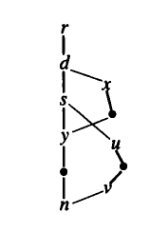
\includegraphics[scale=0.50]{./semidom.png}
\else
\fi
\caption{Semidominator}
\label{fig:1}
\end{center}
\end{figure}

\textbf{Semidominator Theorem}: To find the semidominator of a node \emph{n}, consider all predecessors \emph{v} of \emph{n} in the random graph.
\begin{itemize}
\item If \emph{v} is a proper ancestor of \emph{n} in the spanning tree, \emph{dfnum(v)} $<$ \emph{dfnum(n)}, then \emph{v} is a candidate for \emph{semi(n)}.
\item If \emph{v} is a non-ancestor of \emph{n}, \emph{dfnum(v)} $>$ \emph{dfnum(n)}, then for each \emph{u} that is an ancestor of \emph{v}, or \emph{u} = \emph{v}, \emph{semi(u)} is a candidate for \emph{semi(n)}.
\end{itemize}
Of all these candidates, the one with the lowest \emph{dfnum} is the semidominator of \emph{n}.

\subsection{Dominator Theorem}
On the spanning-tree path below \emph{semi(n)} and above or including \emph{n}, let \emph{y} be the node with the smallest-numbered semidominator (minimum \emph{dfnum(semi(y))}).  Then,
\[
idom(n) = \left\{
\begin{array}{l l}
  semi(n) & \quad \text{if $semi(y) = semi(n)$}\\
  idom(y) & \quad \text{if $semi(y) \neq semi(n)$}\\
\end{array} \right.
\]

\section{Implementation}
The semidominator theorem and dominator theorem have been implemented alongwith depth-first search algorithm.  The dfs(parent, node) assigns the \emph{dfnum} described by the count N.  Also an array \emph{vertex}[N] maps the dfnum back to the nodes.  The array \emph{parent[n]} maintains the parent of each node \emph{n}.  Each node is visited recursively and marked as visited using the \emph{dfnum[n]} array.  A psuedocode for \emph{dfs} routine is given in algorithm 1.

\begin{algorithm}
\caption{Psuedocode for depth-first search routine}
\label{alg1}
\begin{algorithmic}[1]
\STATE \textbf{DFS} (node \emph{p}, node \emph{n})
\IF {\emph{dfnum[n]} = 0}
\STATE \emph{dfnum[n]} $\leftarrow$ N
\STATE \emph{vertex[n]} $\leftarrow$ \emph{n}
\STATE \emph{parent[n]} $\leftarrow$ \emph{p}
\STATE N $\leftarrow$ N + 1
\FOR {each successor \emph{w} of \emph{n}}
\STATE DFS (\emph{n}, \emph{w})
\ENDFOR
\ENDIF
\end{algorithmic}
\end{algorithm}

Link (node$_1$, node$_2$) adds the edge \emph{p} $\rightarrow$ \emph{n} to the spanning forest that is implied by the \emph{ancestor[n]} array.  To find the lowest-numbered semidominator for node \emph{n} other than the root, the function ancestorWithLowestSemi(node \emph{v}) is implemented.  It starts from the rightmost bottom node having the highest \emph{dfnum}, moves up the tree till root, by checking if there exists a lower dfnum for \emph{semi(v)} than the existing one and finally returns the node with lowest-numbered semidominator.  Psuedocodes for Link and ancestorWithLowestSemi routines are given in algorithm 2.

\begin{algorithm}
\caption{Psuedocodes for \emph{Link} and \emph{ancestorWithLowestSemi} routines}
\label{alg2}
\begin{algorithmic}[1]
\STATE /* add edge \emph{p} $\rightarrow$ \emph{n} to spanning forest implied by \emph{ancestor} array */
\STATE \textbf{Link} (node \emph{p}, node \emph{n})
\STATE \emph{ancestor[n]} $\leftarrow$ \emph{p}
\STATE
\STATE /* in a forest, find the nonroot ancestor of \emph{n} that has the lowest-numbered semidominator
\STATE \textbf{ancestorWithLowestSemi} (node \emph{v})
\STATE \emph{u} $\leftarrow$ \emph{v}
\WHILE {\emph{ancestor[v]} $\neq$ none}
\IF {\emph{dfnum[semi[v]]} $<$ \emph{dfnum[semi[u]]}}
\STATE \emph{u} $\leftarrow$ \emph{v}
\ENDIF
\STATE \emph{v} $\leftarrow$ \emph{ancestor[v]}
\ENDWHILE
\STATE \textbf{return} \emph{u}
\end{algorithmic}
\end{algorithm}

The function build$\_$dominator$\_$tree() implements the semidominator and dominator theorem.  If the dominator of \emph{y} is not known, then it is deferred until it is known by using \emph{samedom[n]} array.  Due to this deferring, forests of nodes are created.  Later, with the second clause of dominator theorem, using the samedom array, the forests are linked and the dominators are calculated.  A psuedocode for the building the dominator tree is given in algorithm 3.

\begin{algorithm}
\caption{Psuedocode for build$\_$dominator$\_$tree routine}
\label{alg3}
\begin{algorithmic}[1]
\STATE N $\leftarrow$ 0
\STATE $\forall$\emph{n.bucket[n]} $\leftarrow$ \{\}
\STATE $\forall$\emph{dfnum[n]} $\leftarrow$ 0
\STATE \emph{semi[n]} $\leftarrow$ \emph{ancestor[n]} $\leftarrow$ none
\STATE \emph{idom[n]} $\leftarrow$ \emph{samedom[n]} $\leftarrow$ none
\STATE DFS (none, \emph{r})
\FOR {i $\leftarrow$ N - 1 \textbf{downto} 1}
\STATE \emph{n} $\leftarrow$ \emph{vertex[i]}
\STATE \emph{p} $\leftarrow$ \emph{parent[n]}
\STATE \emph{s} $\leftarrow$ \emph{p}
\FOR {each predecessor \emph{v} of \emph{n}}
\IF {\emph{dfnum[v]} $\leq$ \emph{dfnum[n]}}
\STATE \emph{s'} $\leftarrow$ \emph{v}
\ELSE
\STATE \emph{s'} $\leftarrow$ \emph{semi}[ancestorWithLowestSemi(\emph{v})]
\ENDIF
\IF {\emph{dfnum[s']} $<$ \emph{dfnum[s]}}
\STATE \emph{s} $\leftarrow$ \emph{s'}
\ENDIF
\ENDFOR
\STATE \emph{semi[n]} $\leftarrow$ \emph{s}
\STATE \emph{bucket[s]} $\leftarrow$ \emph{bucket[s]} $\cup$ \{\emph{n}\}
\STATE Link (\emph{p}, \emph{n})
\FOR {each \emph{v} in \emph{bucket[p]}}
\STATE \emph{y} $\leftarrow$ ancestorWithLowestSemi (\emph{v})
\IF {\emph{semi[y]} = \emph{semi[v]}}
\STATE \emph{idom[v]} $\leftarrow$ \emph{p}
\ELSE
\STATE \emph{samedom[v]} $\leftarrow$ \emph{y}
\ENDIF
\ENDFOR
\STATE \emph{bucket[p]} $\leftarrow$ \{\}
\ENDFOR
\FOR {\emph{i} $\leftarrow$ 1 \textbf{to} N - 1}
\STATE \emph{n} $\leftarrow$ \emph{vertex[i]}
\IF {\emph{samedom[n]} $\neq$ none}
\STATE \emph{idom[n]} $\leftarrow$ \emph{idom[samedom[n]]}
\ENDIF
\ENDFOR
\end{algorithmic}
\end{algorithm}
\textbf{Time Complexity}:  The routine AncestorWithLowestSemi(node \emph{v}) starts from a node with highest \emph{dfnum} (the rightmost bottom node) and runs through the entire graph upto the root taking a O(N) time, N being the total number of nodes in the graph.  The dominator routine implements Langauer-Tarjan algorithm taking O(N) time, the linear time.  Thus, the complexity of the entire algorithm is O(N$_2$).  If we can achieve a complexity of O(log N) with ancestorWithLowestSemi() by path compression techniques, then the complexity reduces to O(N log N).

\section{Sample Run}
\begin{figure}[htb]
\begin{center}
\ifpdf
	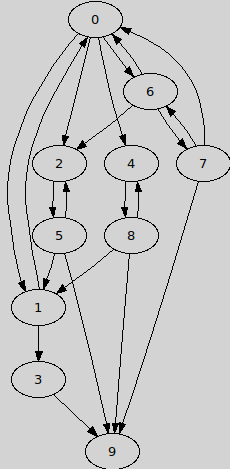
\includegraphics[scale=0.50]{./cfg.png}
\else
\fi
\caption{Some randomly generated graph}
\label{fig:2}
\end{center}
\end{figure}

\begin{figure}[htb]
\begin{center}
\ifpdf
	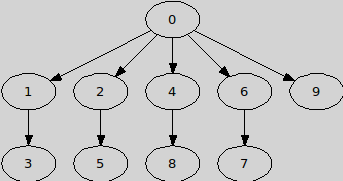
\includegraphics[scale=0.50]{./dom.png}
\else
\fi
\caption{Dominator tree for figure 2}
\label{fig:3}
\end{center}
\end{figure}
Figure 2 shows a randomly generated graph.  After running through the Lenguer-Tarjan algorithm for dominator computation, a dominator tree shown in figure 3 was generated.  The root node was considered to be at node 0.

\begin{thebibliography}{10}
\bibitem {appel}{appel} andrew w. appel, \emph{modern compiler implementation in c}, Revised Edition, Cambridge University Press, 2008
\end{thebibliography}

\end{document}